\documentclass[10pt]{article}
\usepackage{polski}
\usepackage[left=1cm, right=1.5cm, top=0cm, bottom=1cm]{geometry}
\usepackage{multicol}
% \renewcommand{\familydefault}{\sfdefault}
\usepackage{lipsum}
\usepackage{graphicx}
\usepackage[T1]{fontenc}
\usepackage{charter}
\usepackage{enumitem}
\usepackage{fancyvrb}
\usepackage{nopageno}
\usepackage[dvipsnames]{xcolor}

\begin{document}

    % \hskip-1.55cm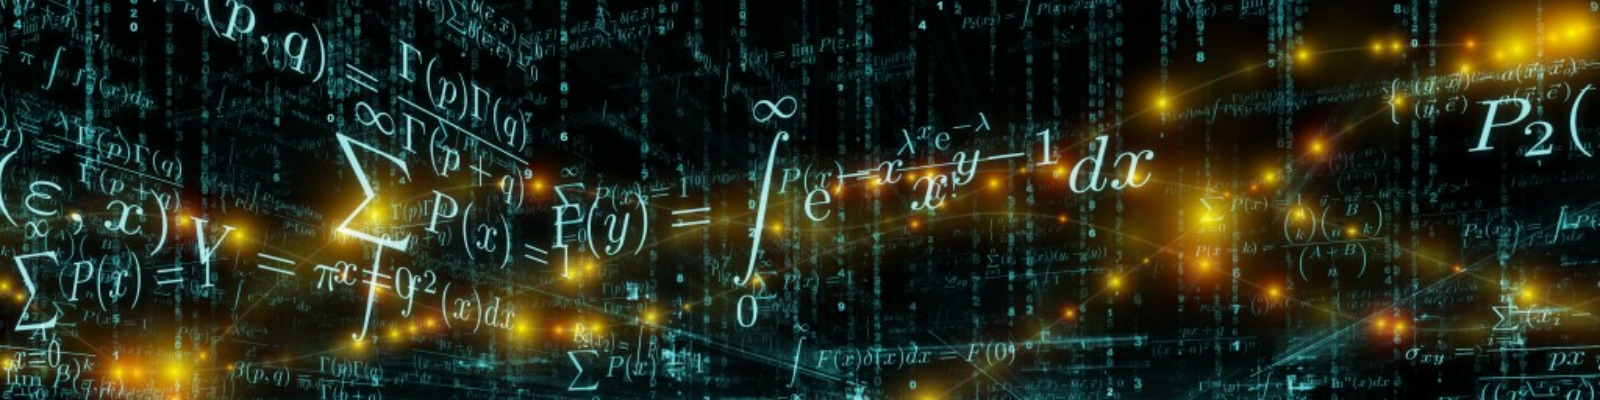
\includegraphics[scale=0.4]{banner.png}
    % \hskip-1.55cm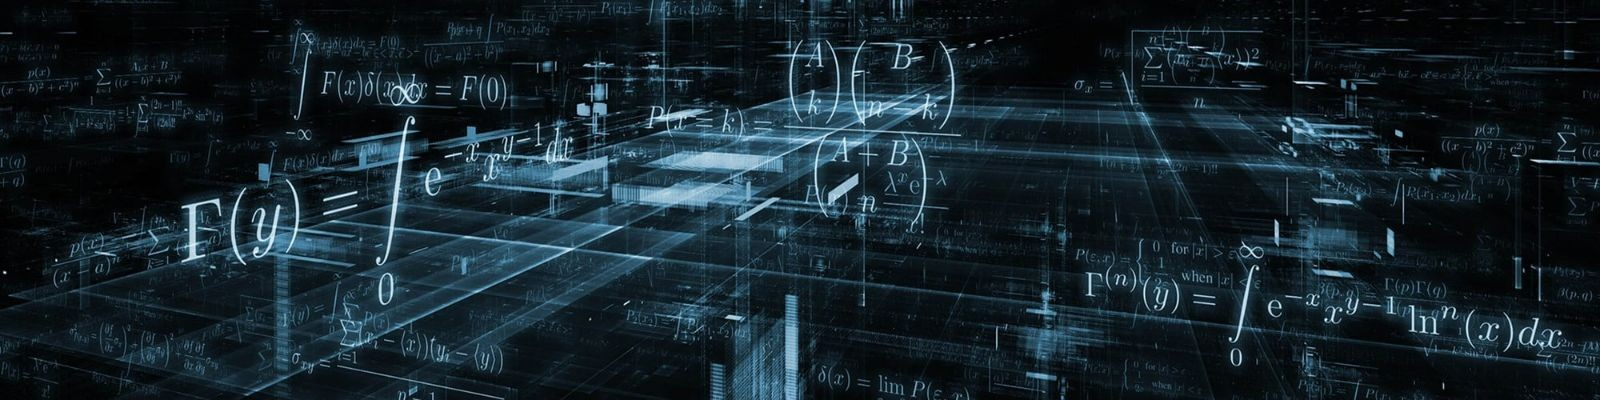
\includegraphics[scale=1.6]{banner4.jpg}
    \hskip-1.55cm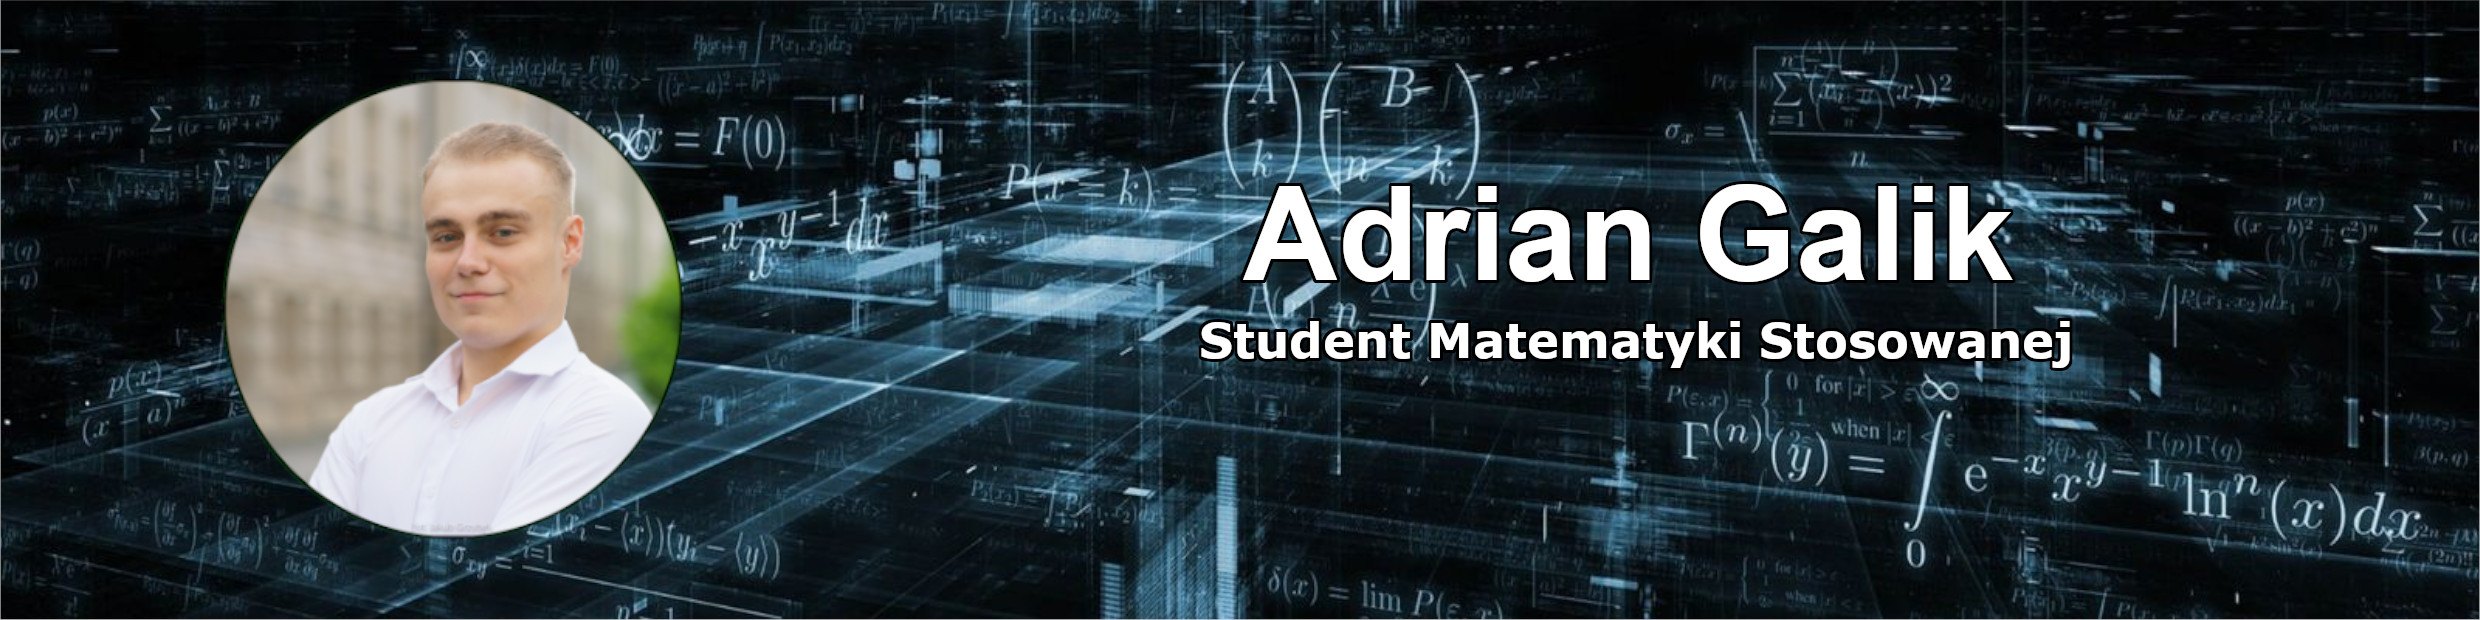
\includegraphics[scale=0.245]{benger.jpg}
    % \hskip-1.55cm
\includegraphics[scale=1.6]{banner5.jpg}
    % \hskip-1.6cm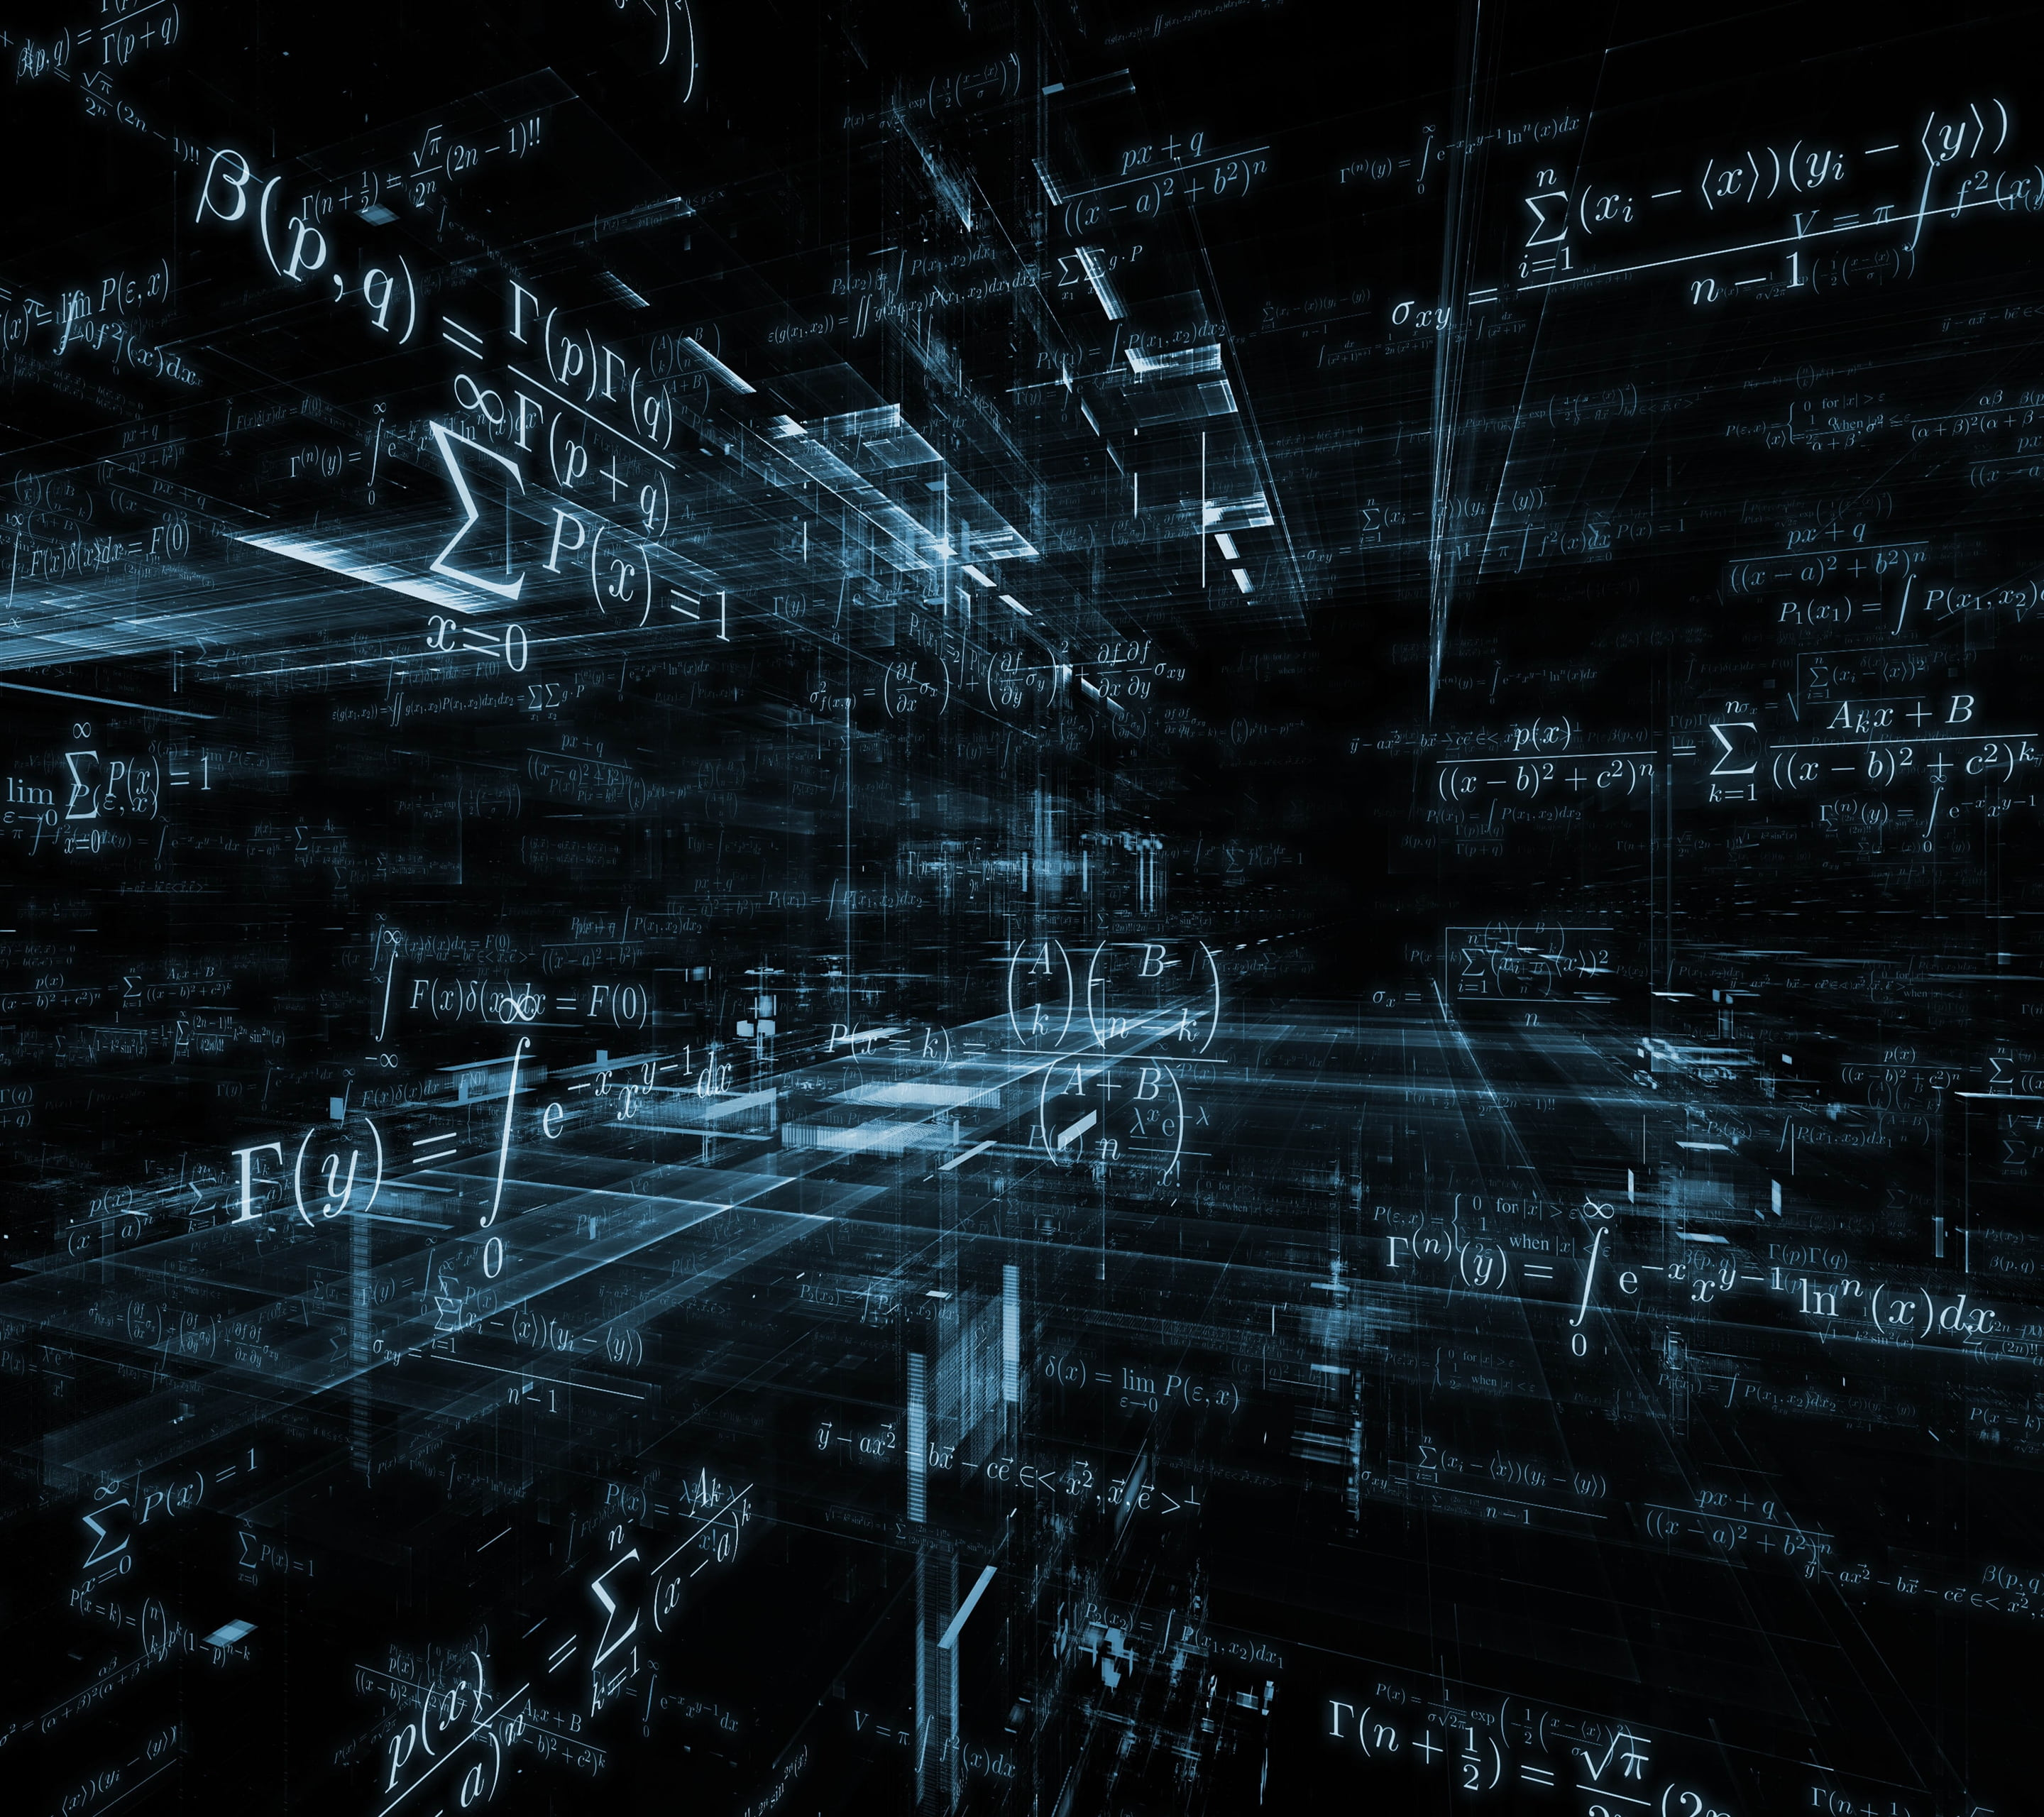
\includegraphics[height=0.20\textheight, width=1.5\textwidth]{banner2.jpg}
    % \hskip-1.6cm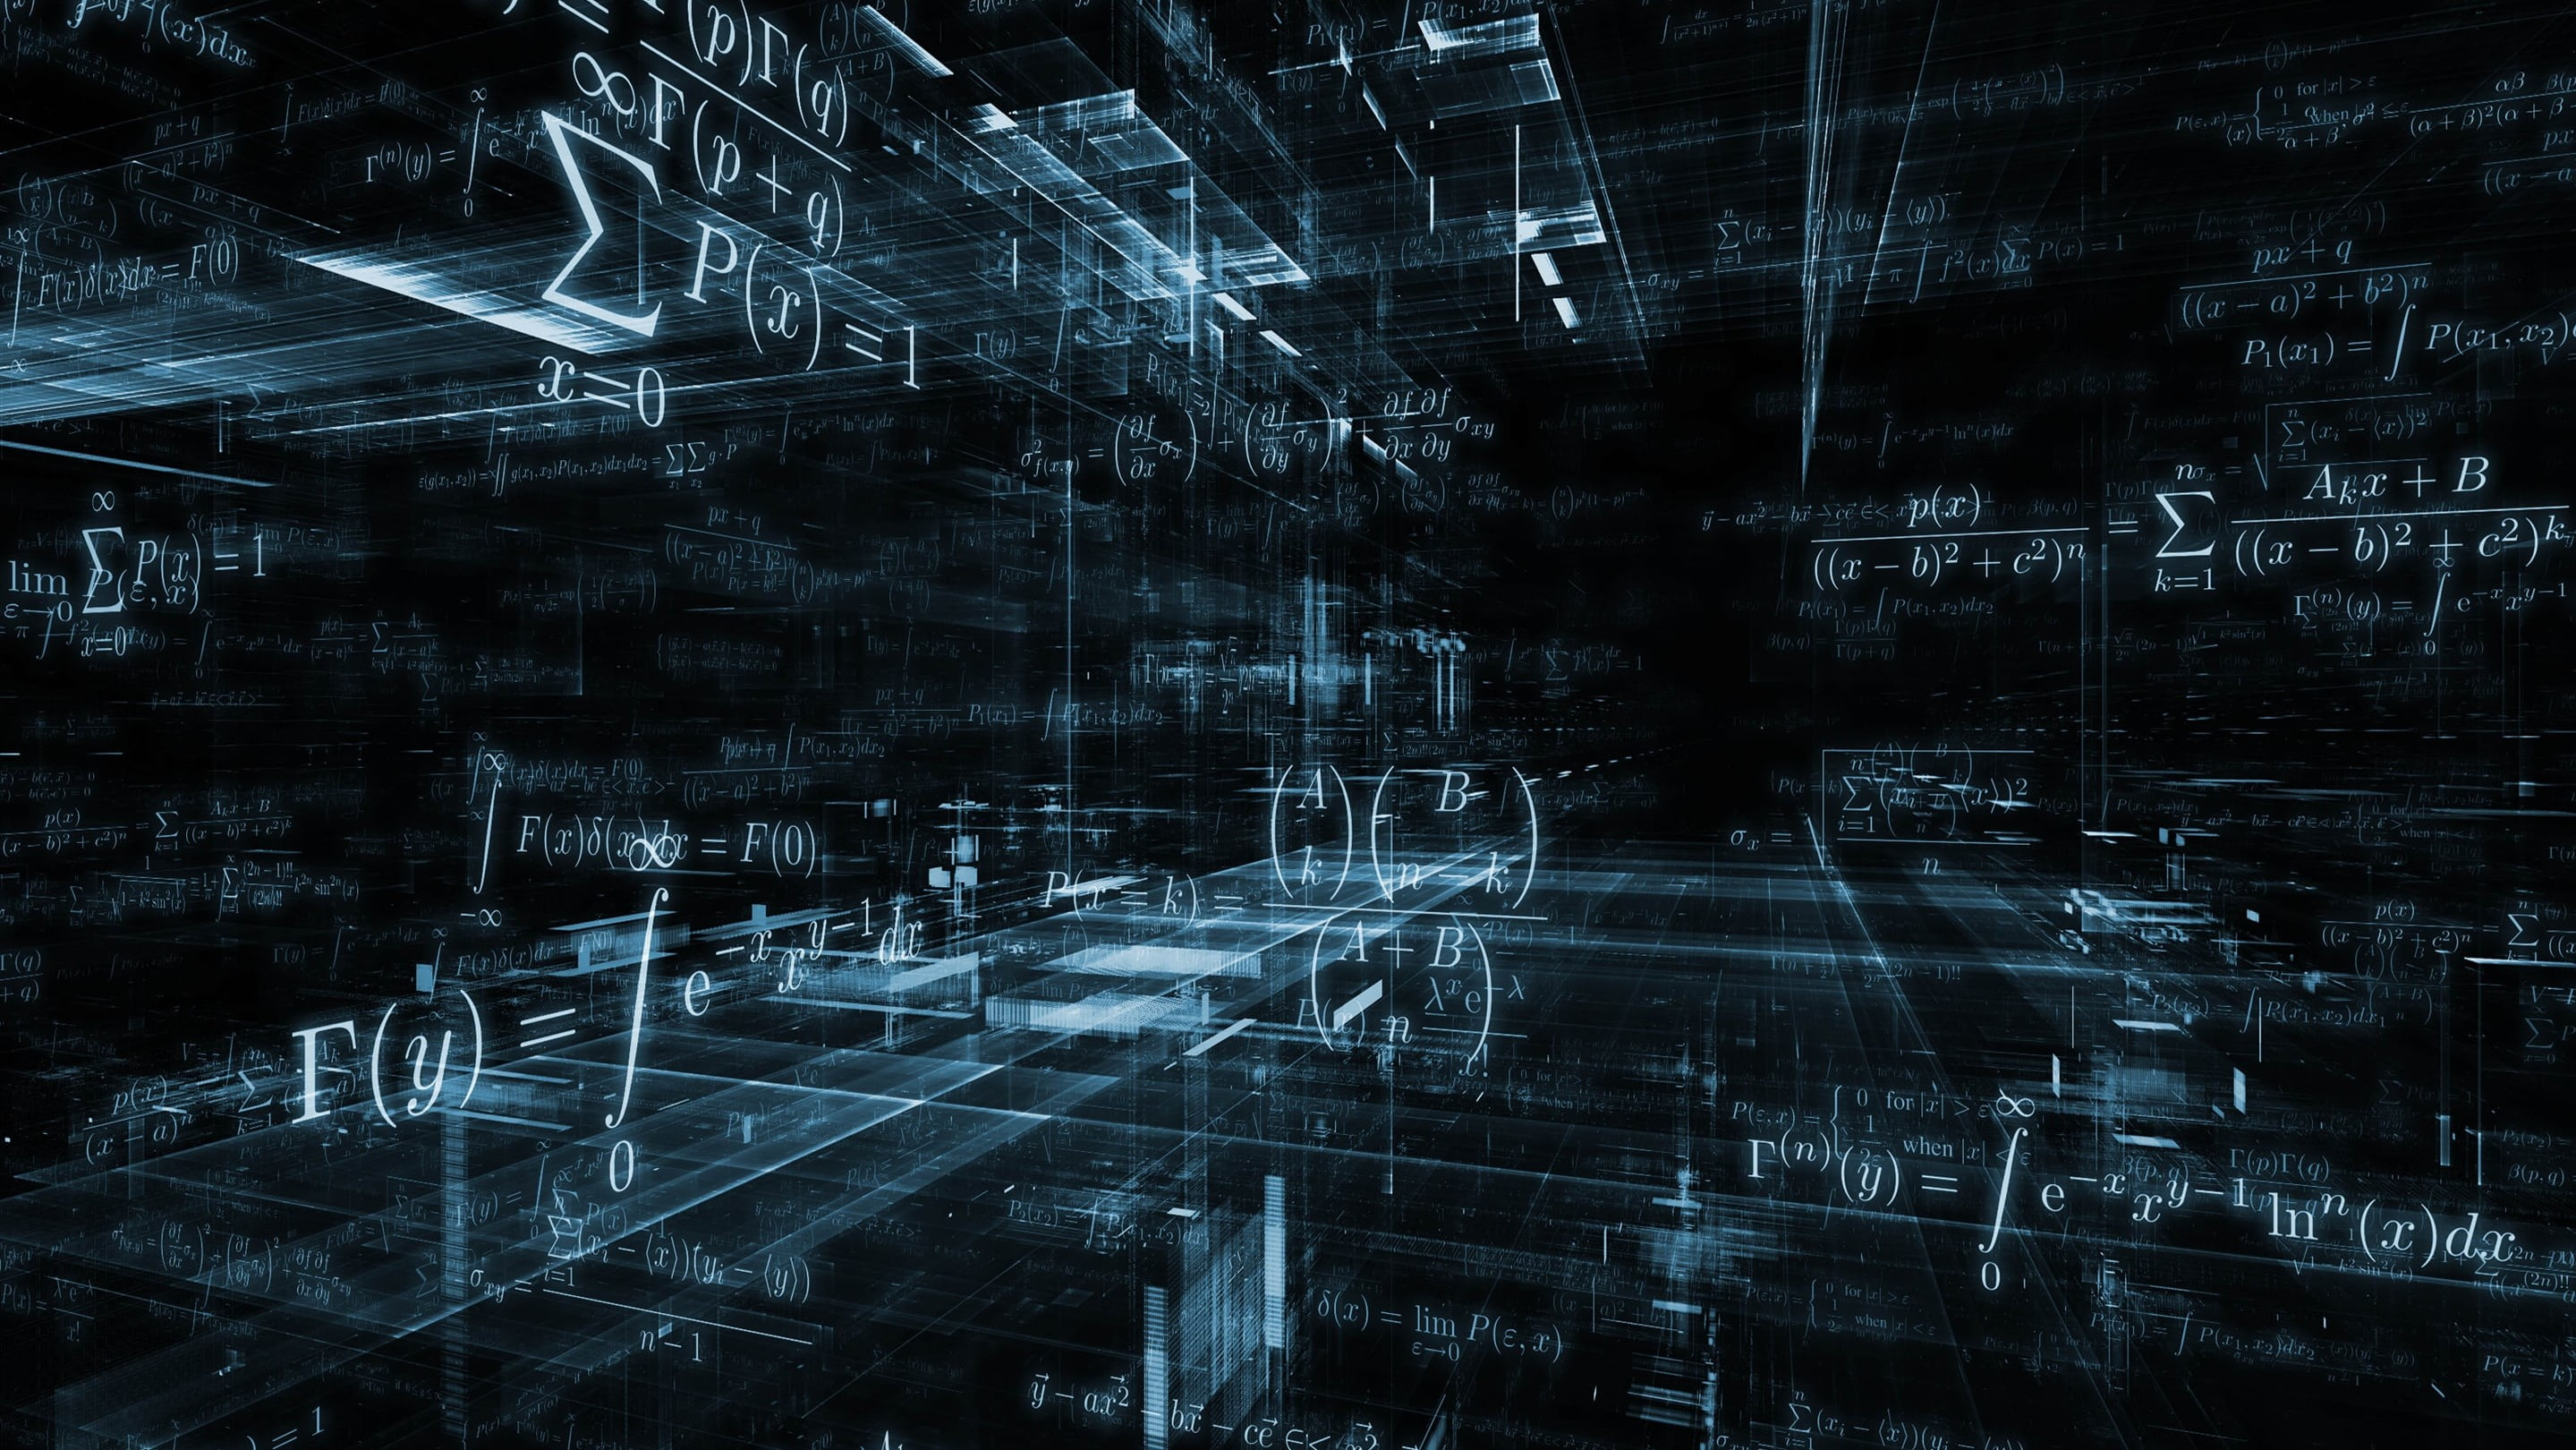
\includegraphics[height=0.25\textheight, width=1.5\textwidth]{banner3.jpg}
    \noindent
    \thispagestyle{empty}

    \vskip+0.4cm\begin{minipage}[t]{0.30\textwidth}
        \textbf{+48 663 383 000 \\
        adrian1galik@gmail.com \\
        github.com/Vexus1} \\
        \rule{6cm}{1pt} \\ \\
        \fontsize{14pt}{14pt}{\textbf{\color{Violet}UMIEJĘTNOŚCI:}}
        \fontsize{10pt}{10pt}
        \begin{itemize}[leftmargin=*]
            \setlength{\parskip}{0pt}
            % \setlength\itemsep{0pt} 
            \item \textbf{Python} poziom średnio \\ zaawansowany
            \item Biblioteki programistyczne: \raggedright \\ \textbf{NumPy, Pandas, OpenCV, TensorFlow, Keras, ROS2}
            \item Abstrakcyjne struktury danych: \textbf{Stosy, Kolejki, Drzewa, Grafy}
            \item Zarządzanie bazami danych: \textbf{SQL}
            \item Modele i metody statystyki \\ matematczynej \textbf{język R}
            % \item Wizualizacja danych \textbf{Power BI}
            \item Tworzenie i administrowanie \\ stronami internetowymi: \textbf{HTML, CSS, JavaScript, React, Flask, PHP}
            % \item Zastosowanie równań \\ różniczkowych
            \item Projektowanie i zarządzanie \\ sieciami komputerowymi
            \item System kontroli wersji: \textbf{Git}
            % \item Tworzenie i administrowanie \\ stronami internetowymi: \textbf{HTML, CSS, JavaScript, Flask, PHP}
            \item System operacyjny: \textbf{Linux}
            % \item Język formatowania tekstu: \textbf{LaTeX}
            \item Obliczenia numeryczne: \textbf{Julia}
            \item Powłoka systemowa UNIX: \textbf{Bash} 
            \item Środowisko tworzenia aplikacji: \textbf{Docker}
            \item Analityczne myślenie
            % \item Praca zespołowa 
        \end{itemize}
        \rule{6cm}{1pt} \\ \\
        \fontsize{14pt}{14pt}{\textbf{\color{Violet}JĘZYKI:}}
        \fontsize{10pt}{10pt}
        \begin{itemize}[leftmargin=*]
            \setlength{\parskip}{0pt}
            % \setlength\itemsep{0pt} 
            \item Polski ojczysty
            \item Angielski C1
        \end{itemize}
        \rule{6cm}{1pt} \\ \\
        \fontsize{14pt}{14pt}{\color{Violet}\textbf{ZAINTERESOWANIA:}}
        \fontsize{10pt}{10pt}
        \begin{itemize}[leftmargin=*]
            \setlength{\parskip}{0pt}
            % \setlength\itemsep{0pt} 
            \item Uczenie maszynowe
            \item Matematyka
            \item Astrofizyka
        \end{itemize}
    \end{minipage}
    \hfill % horizontal space between columns
    \begin{minipage}[t]{0.60\textwidth}
        \fontsize{14pt}{14pt}{\textbf{\color{Violet}O MNIE:}}
        \fontsize{10pt}{10pt}
        \\


        Ambitny student \textbf{Matematyki Stosowanej}. Wykorzystuje więdzę matematyczną 
        do pisania algorytmów związanych ze \textbf{sztuczną inteligencją}, 
        głównie \textbf{uczeniem maszynowym}. Moim ulubionym językiem
        programowania jest \textbf{Python} i chciałbym go wykorzystywać w swojej pracy.
        W przyszłości widzę siebie w obszarze \textbf{uczenia maszynowego}. \\ \\
        \rule{11cm}{1pt} \\ \\
        \fontsize{14pt}{14pt}{\textbf{\color{Violet}DOŚWIADCZENIE:}}
        \fontsize{10pt}{10pt}
        \begin{itemize}[leftmargin=*]
            \setlength{\parskip}{0pt}
            % \setlength\itemsep{0pt} 
            \item Koło naukowe \textbf{Robocik} działające na Politechnice Wrocławskiej. \\
            Projektowanie \textbf{sztucznej inteligencji}, pisanie algorytmów do \\
            wykrywania położenia drona podwodnego i obsługi sterowania w \\ technologi \textbf{ROS2 (Python)},
            pod zagraniczne zawody \textbf{TAC Challange}.
            % Przygotowanie, rozwój i walidacja zautomatyzowanych testów \\
            % funkcjonalności uruchamianych podczas przygotowania drona do \\
            % pływania (\textbf{Python OpenCV})
            \item Projekty programistycznie w języku \textbf{Python} tj. gra 2D napisana \\
            w paradygmacie obiektowym przy użyciu biblioteki \textbf{Pygame} \\
            numerczyne rozwiązanie równania różniczkowego Friedmana \\
            określającego ewolucję wszechświata  (\textbf{github})
            \item Praktyki zawodowe w firmie \textbf{Sports Media}. Sieci i systemy \\ komputerowe
            \item Praktyki zawodowe w firmie \textbf{Zapaśnik IT}. Zarządzanie systemami  \\komputerowymi
            \item Członek komisji do spraw Dydaktyki i Praw Studenta
            % \item Projekt symulujący układ słoneczny (odziaływania grawitacyjne) \\ poprzez numeryczne rozwiązywanie problemu n-ciał  (\textbf{Python})
            % \item Projekt rozwiązujący numerczynie (bez użycia bibliotek) równania różniczkowe Friedmana określające ewolucję wszechświata.
            % Celem było uzyskanie informacji o wszechświecie tj. wiek, przeszły i przyszły jego rozwój (\textbf{Python})
        \end{itemize}
        \rule{11cm}{1pt} \\ \\
        \fontsize{14pt}{14pt}{\textbf{\color{Violet}WYKSZTAŁCENIE:}}
        \fontsize{10pt}{10pt}
        \begin{itemize}[leftmargin=*]
            \setlength{\parskip}{0pt}
            % \setlength\itemsep{0pt} 
            \item \textbf{Politechnika Wrocławska, Matematyka Stosowana, Studia \\ inżynierskie, październik 2021 - nadal}
            \item \textbf{Zespół Szkół Teleinformatycznych i Elektronicznych we Wrocławiu, Technikum nr 7, Technik Informatyk, wrzesień 2017 - kwiecień 2021} 
        \end{itemize}
        \rule{11cm}{1pt} \\ \\
        \fontsize{14pt}{14pt}{\textbf{\color{Violet}CERTYFIKATY:}}
        \fontsize{10pt}{10pt}
        \begin{itemize}[leftmargin=*]
            \setlength{\parskip}{0pt}
            % \setlength\itemsep{0pt} 
            \item \textbf{Kwalifikacja EE.09 - Programowanie, tworzenie i administrowanie stronami
            internetowymi i bazami danych}
            \item \textbf{Kwalifikacja EE.08 - Montaż i eksploatacja systemów komputerowych, urządzeń
            peryferyjnych i sieci}
        \end{itemize}
        \rule{0pt}{0pt} \\ \\ \\
        \fontsize{7pt}{5pt}\selectfont  
        Wyrażam zgodę na przetwarzanie moich danych osobowych zawartych w dokumentach aplikacyjnych w
        celu przeprowadzenia postępowania rekrutacyjnego.
        Wyrażam zgodę na przetwarzanie moich danych osobowych w celu wykorzystania ich w kolejnych
        prowadzonych naborach przez okres najbliższych 12 miesięcy
    \end{minipage}

\end{document}